\documentclass[12pt, a4paper, oneside]{ctexart}
\usepackage{amsmath, amsthm, amssymb, bm, color, graphicx, geometry, mathrsfs,extarrows, braket, booktabs, array}
\usepackage[colorlinks,linkcolor=red,anchorcolor=blue,citecolor=blue,urlcolor=blue,menucolor=black]{hyperref}
\setCJKmainfont{方正新书宋_GBK.ttf}[BoldFont=方正小标宋简体, ItalicFont=方正楷体_GBK]
\setmainfont{Times New Roman}  % 设置英文字体
\setsansfont{Calibri}
\setmonofont{Consolas}

\linespread{1.4}
%\geometry{left=2.54cm,right=2.54cm,top=3.18cm,bottom=3.18cm}
\geometry{left=1.84cm,right=1.84cm,top=2.18cm,bottom=2.18cm}
\newcounter{problem}  % 问题序号计数器
\newcounter{problem*}  % 问题序号计数器
\newenvironment{problem}{\stepcounter{problem}\par\noindent\textbf{题目\arabic{problem}. }}{\smallskip\par}
\newenvironment{problem*}{\stepcounter{problem*}\par\noindent\textbf{编程作业\arabic{problem*}. }}{\smallskip\par}
\newenvironment{solution}{\par\noindent\textbf{解答. }}{\smallskip\par}
\newenvironment{note}{\par\noindent\textbf{注记. }}{\smallskip\par}

%%%% 图片相对路径 %%%%
\graphicspath{{figure/}} % 当前目录下的figure文件夹, {../figure/}则是父目录的figure文件夹
\setlength{\abovecaptionskip}{-0.2cm}  % 缩紧图片标题与图片之间的距离
\setlength{\belowcaptionskip}{0pt} 

\everymath{\displaystyle} % 默认全部行间公式
\DeclareMathOperator*\uplim{\overline{lim}} % 定义上极限 \uplim_{}
\DeclareMathOperator*\lowlim{\underline{lim}} % 定义下极限 \lowlim_{}
\let\leq=\leqslant % 将全部leq变为leqslant
\let\geq=\geqslant % geq同理
\DeclareRobustCommand{\rchi}{{\mathpalette\irchi\relax}}  % \rchi中间位置的\chi
\newcommand{\irchi}[2]{\raisebox{\depth}{$#1\chi$}} % inner command, used by \rchi

%%%% 一些宏定义 %%%%
\def\bd{\boldsymbol}        % 加粗(向量) boldsymbol
\def\disp{\displaystyle}    % 使用行间公式 displaystyle(默认)
\def\tsty{\textstyle}       % 使用行内公式 textstyle
\def\sign{\text{sign}}      % sign function
\def\wtd{\widetilde}        % 宽波浪线 widetilde
\def\R{\mathbb{R}}          % Real number
\def\N{\mathbb{N}}          % Natural number
\def\Z{\mathbb{Z}}          % Integer number
\def\Q{\mathbb{Q}}          % Rational number
\def\C{\mathbb{C}}          % Complex number
\def\d{\mathrm{d}}          % differential operator
\def\e{\mathrm{e}}          % Euler's number
\def\i{\mathrm{i}}          % imaginary number
\def\re{\mathrm{Re}}        % Real part
\def\im{\mathrm{Im}}        % Imaginary part
\def\res{\mathrm{Res}}      % Residue
\def\L{\mathcal{L}}         % Loss function
\def\wdh{\widehat}          % 宽帽子 widehat
\def\ol{\overline}          % 上横线 overline
\def\ul{\underline}         % 下横线 underline
\def\add{\vspace{1ex}}      % 增加行间距
\def\del{\vspace{-3.5ex}}   % 减少行间距

%%%% 定理类环境的定义 %%%%
\newtheorem{theorem}{定理}

%%%% 基本信息 %%%%
\newcommand{\RQ}{\today} % 日期
\newcommand{\km}{数理统计} % 科目
\newcommand{\bj}{强基数学002} % 班级
\newcommand{\xm}{吴天阳} % 姓名
\newcommand{\xh}{2204210460} % 学号

\begin{document}

%\pagestyle{empty}
\pagestyle{plain}
\vspace*{-15ex}
\centerline{\begin{tabular}{*5{c}}
    \parbox[t]{0.25\linewidth}{\begin{center}\textbf{日期}\\ \large \textcolor{blue}{\RQ}\end{center}} 
    & \parbox[t]{0.2\linewidth}{\begin{center}\textbf{科目}\\ \large \textcolor{blue}{\km}\end{center}}
    & \parbox[t]{0.2\linewidth}{\begin{center}\textbf{班级}\\ \large \textcolor{blue}{\bj}\end{center}}
    & \parbox[t]{0.1\linewidth}{\begin{center}\textbf{姓名}\\ \large \textcolor{blue}{\xm}\end{center}}
    & \parbox[t]{0.15\linewidth}{\begin{center}\textbf{学号}\\ \large \textcolor{blue}{\xh}\end{center}} \\ \hline
\end{tabular}}
\begin{center}
    \zihao{-3}\textbf{第二次作业}
\end{center}
\vspace{-0.2cm}
% 正文部分
\begin{problem}
    设$X_1, \cdots, X_n$来自$N(0,1)$的随机样本,令
    \begin{equation*}
        \bar{X}_k=\frac{1}{k}\sum_{i=1}^kX_i,\quad\bar{X}_{n-k}=\frac{1}{n-k}\sum_{i=k+1}^nX_i,
    \end{equation*}
    求下列分布:(1) $\frac{1}{2}(\bar{X}_k+\bar{X}_{n-k})$. (2) $k\bar{X}_k^2+(n-k)\bar{X}_{n-k}^2$. (3) $X_1^2/X_2^2$. (4) $X_1/X_n$.
\end{problem}
\begin{solution}
    (1) $\bar{X}_k\sim N(0,\frac{1}{k}),\ \bar{X}_{n-k}\sim N(0,\frac{1}{n-k})$,所以$\frac{\bar{X}_k+\bar{X}_{n-k}}{2} \sim(0,\frac{1}{4}(\frac{1}{k}+\frac{1}{n+k}))$.\add

    (2) $\sqrt{k}\bar{X}_k\sim N(0,1),\ \sqrt{n-k}\bar{X}_{n-k}\sim N(0,1)$,所以$k\bar{X}_k^2+(n-k)\bar{X}_{n-k}^2\sim \rchi(2)$.\add

    (3) $X_1^2,\ X_2^2\overset{iid}{\sim} \rchi(1)$,所以$\frac{X_1^2}{X_2^2}\sim F(1,1)$.

    (4) 设$U = X_1/X_2, V = X_2$,于是$x_1 = uv, x_2 = v$,$\det(J) = \left|\begin{matrix}
        v&u\\0&1
    \end{matrix}\right| = v$,且$p_{X_1,X_2}(x_1,x_2) = \frac{1}{2\pi}\e^{-\frac{x_1^2+x_2^2}{2}}$,则
    \begin{equation*}
        p_{U,V}(u, v) = P_{X_1,X_2}(uv, v)|v| = \frac{1}{2\pi}\e^{-\frac{u^2v^2+v^2}{2}}|v| = \frac{|v|}{2\pi}\e^{-\frac{v^2(u^2+1)}{2}},
    \end{equation*}
    则
    \begin{equation*}
        P_{X_1/X_2}(u) = P_U(u) = 2\int_0^\infty \frac{v}{2\pi}\e^{-\frac{v^2(u^2+1)}{2}}\,\d v = \frac{1}{\pi(u^2+1)},
    \end{equation*}
    所以$U\sim \text{Cauchy}(0,1)$为标准Cauchy分布.
\end{solution}
\begin{problem}
    设$X_1,\cdots, X_n$是来自双参数指数分布
    \begin{equation*}
        f(x,\mu,\sigma)=\frac{1}{\sigma}\exp\left\{-\frac{x-\mu}{\sigma}\right\},\quad x \geq \mu
    \end{equation*}
    的简单随机样本,其中$u\in \R, \sigma >0$,求$\mu,\sigma$和$P(X_1\geq t),\ (t > \mu)$的矩估计和MLE.
\end{problem}
\begin{solution}
    矩估计:由于
    \begin{align*}
        E(X) =&\ \int_\mu^\infty\frac{x}{\sigma}\exp\left\{-\frac{x-\mu}{\sigma}\right\}\,\d x =\frac{1}{\sigma}\left(\int_0^\infty x\e^{\frac{x}{\sigma}}+\mu\e^{-\frac{x}{\sigma}}\right)\,\d x \xlongequal{\text{凑Gamma分布}}\sigma+\mu\\
        E(X^2) =&\ \int_\mu^\infty\frac{x^2}{\sigma}\exp\left\{-\frac{x-\mu}{\sigma}\right\}\,\d x = \frac{1}{\sigma}\left(\int_0^\infty x^2\e^{-\frac{x}{\sigma}}+2\mu\int_0^\infty x\e^{-\frac{x}{\sigma}}+\mu^2\int_0^\infty\e^{-\frac{x}{\sigma}}\right)\,\d x\\
        &\hspace{-0.5cm} \xlongequal{\text{凑Gamma分布}}2\sigma^2+2\mu\sigma+\mu^2
    \end{align*}
    则$\mu,\sigma$的矩估计为
    \begin{equation*}
        \begin{cases}
            \bar{X} = \sigma+\mu,\\
            M_2' = 2\sigma^2+2\mu\sigma+\mu^2.
        \end{cases}\Rightarrow\quad\begin{cases}
            \hat{\mu}=\bar{X}-\sqrt{M_2'-\bar{X}^2},\\
            \hat{\sigma} = \sqrt{M_2'-\bar{X}^2}.
        \end{cases}
    \end{equation*}
    于是$P(X_1\geq t)$的矩估计为
    \begin{equation*}
        P(X_1\geq t) = \int_t^\infty\frac{1}{\sigma}\exp\left\{-\frac{x-\mu}{\sigma}\right\}\,\d x=\sqrt{\frac{\pi}{\sigma}}\int_{t-\mu}^\infty\frac{1}{\sqrt{\pi\sigma}}\exp\left\{-\frac{x}{\sigma}\right\}\,\d x=\sqrt{\pi}{\hat{\sigma}}(1-\Phi(t-\hat{\mu})).
    \end{equation*}

    MLE:似然函数$L(\mu,\sigma) = \prod_{i=1}^n\frac{1}{\sigma}\exp\left\{-\frac{x_i-\mu}{\sigma}\right\} = \frac{1}{\sigma^n}\exp\left\{-\frac{\sum_{i=1}^nx_i-n\mu}{\sigma}\right\}$,对数似然为$\log L(\mu,\sigma) = -n\log\sigma-\frac{1}{\sigma}\left(\sum_{i=1}^nx_i-n\mu\right)$,但方程$\frac{\partial \log L}{\partial\mu} = \frac{n}{\sigma} = 0$无解,所以该分布不存在MLE.
\end{solution}
\begin{problem}
    设$X_1,\cdots,X_n$和$Y_1,\cdots, Y_n$分别来自正态总体$N(\mu_1,\sigma^2)$和$N(\mu_2,\sigma^2)$的随机样本,求$\mu_1,\mu_2,\sigma^2$的MLE.
\end{problem}
\begin{solution}
    似然函数为$L(\mu_1,\mu_2,\sigma) = \prod_{i=1}^n\frac{1}{\sqrt{2\pi}\sigma}\e^{-\frac{(x_i-\mu_1)^2}{2\sigma^2}}\prod_{j=1}^n\frac{1}{\sqrt{2\pi}\sigma}\e^{-\frac{(y_j-\mu_2)^2}{2\sigma^2}}$,对数似然为$\log L(\mu_1,\mu_2,\sigma^2)=-2n\log(\sqrt{2n\sigma^2})-\frac{1}{2\sigma^2}\left(\sum_{i=1}^n(x_i-\mu_1)^2+\sum_{j=1}^n(y_j-\mu_2)^2\right)$,于是
    \begin{equation*}
        \begin{cases}
            \frac{\partial \log L}{\partial \mu_1} = \frac{1}{\sigma^2}\sum_{i=1}^n(x_i-\mu_1)=0,\\
            \frac{\partial \log L}{\partial \mu_2} = \frac{1}{\sigma^2}\sum_{j=1}^n(y_i-\mu_2)=0,\\
            \frac{\partial \log L}{\partial \sigma} = -\frac{n}{\sigma^2}+\frac{1}{2\sigma^4}\left(\sum_{i=1}^n(x_i-\mu_1)^2+\sum_{j=1}^n(y_j-\mu_2)^2\right)=0.
        \end{cases}\hspace{-1cm}\Rightarrow\begin{cases}
            \hat{\mu}_1 = \frac{1}{n}\sum_{i=1}^nx_i = \bar{X},\\
            \hat{\mu}_2 = \frac{1}{n}\sum_{i=1}^ny_i = \bar{Y},\\
            \hat{\sigma}^2=\frac{1}{2n}\left(\sum_{i=1}^n(x_i-\hat{\mu}_1)^2+\sum_{j=1}^n(y_j-\mu_2)^2\right).
        \end{cases}
    \end{equation*}
\end{solution}
\begin{problem}
    设$X_1,\cdots, X_n$来自均匀分布$U(\theta,2\theta)$的随机样本,其中$\theta>0$,求:(1) $\theta$的MLE $\hat{\theta}$;(2) 判断$\hat{\theta}$是否是无偏估计,如果不是无偏估计,基于$\hat{\theta}$构造一个无偏估计.
\end{problem}
\begin{solution}
    (1) 似然函数$L(\theta) = \frac{1}{\theta}\prod_{i=1}^nI_{[\theta,2\theta]}(x_i)$,令$Y_1,\cdots,Y_n$为$X_1,\cdots,X_n$的次序统计量,\add 则$L(\theta)=1$时,有$y_1\geq \theta, y_n\leq 2\theta\Rightarrow \frac{y_n}{2}\leq \theta\leq y_1$. 则$L(\theta) = \frac{1}{\theta}I_{[\frac{y_n}{2},y_1]}(\theta)$,因此$\hat{\theta} = \frac{y_n}{2}$.

    (2) 由于$F_{Y_n}(y) = P(X_1,\cdots,X_n\leq y) = (F_X(y))^n = (\frac{y-\theta}{\theta})^{n},\ y\in [\theta, 2\theta]$,于是
    \begin{equation*}
        f_{Y_n}(y) = \frac{n}{\theta}(\frac{y-\theta}{\theta})^{n-1}I_{[\theta,2\theta]}(y)
    \end{equation*}
    则
    \begin{equation*}
        E(\hat{\theta})=E(\frac{y_n}{2})=\frac{1}{2}\int_\theta^{2\theta}y \frac{n}{\theta}(\frac{y-\theta}{\theta})^{n-1}\,\d y=\frac{n}{2\theta^n}\int_0^\theta(y+\theta)y^{n-1}\,\d y = \frac{2n+1}{2n+2}\theta.
    \end{equation*}
    所以$\hat{\theta}$为$\theta$的有偏估计,构造$\hat{\theta}'  =\frac{2n+2}{2n+1}\hat{\theta} = \frac{n+1}{2n+1}y_n$是$\theta$的无偏估计.
\end{solution}
\begin{problem}
    设$X$服从对数正态分布,即$\ln X\sim N(\mu,\sigma^2)$,其中$\mu\in \R,\sigma >0$. 设$X_1,\cdots, X_n$来自总体$X$的随机样本,求:(1) $\mu,\sigma^2$的MLE;(2) 求$E(X)$的MLE.
\end{problem}
\begin{solution}
    (1) 令$Y = \log X$,则$f_X(x) = f_Y(\log x)\frac{1}{x} = \frac{1}{x\sqrt{2\pi}\sigma}\e^{-\frac{(\log x-\mu)^2}{2\sigma^2}}$,则似然函数
    \begin{align*}
        L(\mu,\sigma^2) =&\ \prod_{i=1}^nf(x_i) = \frac{1}{(\sqrt{2\pi\sigma^2})^2\prod_{i=1}^nx_i}\e^{-\frac{1}{2\sigma^2}\sum_{i=1}^n(\log x_i-\mu)^2},\\
        \Rightarrow\ \log L(\mu,\sigma^2)=&\ -\frac{n}{2}\log(2\pi\sigma^2)-\sum_{i=1}^n\log(x_i)-\frac{1}{2\sigma^2}\sum_{i=1}^n(\log x_i-\mu)^2.
    \end{align*}
    于是
    \begin{equation*}
        \begin{cases}
            \frac{\partial \log L}{\partial \mu} = \frac{1}{\sigma^2}\sum_{i=1}^n(\log x_i-\mu) = 0,\\
            \frac{\partial \log L}{\partial \sigma^2} = -\frac{n}{2\sigma^2}+\frac{1}{2\sigma^4}\sum_{i=1}^n(\log x_i-\mu)^2=0.
        \end{cases}\Rightarrow\quad\begin{cases}
            \hat{\mu} = \frac{1}{n}\sum_{i=1}^n\log x_i,\\
            \hat{\sigma}^2 = \frac{1}{n}\sum_{i=1}^n(\log x_i-\hat{\mu})^2.
        \end{cases}
    \end{equation*}

    (2) $E(X)$的MLE为
    \begin{align*}
        E(x) =&\ \int_0^\infty \frac{1}{\sqrt{2\pi}\sigma}\e^{-\frac{(\log x-\mu)^2}{2\sigma^2}}\,\d x = \int_R\frac{1}{\sqrt{2\pi}\sigma}\e^{-\frac{(x-\mu)^2-2\sigma^2x}{2\sigma^2}}\,\d x\\
        \xlongequal{\text{凑Gauss分布}}&\ \frac{1}{\sqrt{2\pi\hat{\sigma}^2}}\e^{2\hat{\mu}+\hat{\sigma}^2}.
    \end{align*}
\end{solution}
\begin{problem*}
    假设$X_1,\cdots, X_n$是来自总体$X$的随机样本,$X\sim\rchi^2(k)$.
    
    (1) 求样本均值$\bar{X}$的密度函数.

    (2) 求样本均值的渐近分布.

    (3) 通过编程比较,在不同样本量下,样本均值的密度函数和其渐近分布的密度函数图像.
\end{problem*}
\begin{solution}
    (1) $n\bar{X} = \sum_{i=1}^nX_i$,由于$X_i\sim \rchi(k) = \Gamma(\frac{k}{2}, \frac{1}{2})$,且Gamma函数有可加性,则$N\bar{X}\sim\Gamma(\frac{nk}{2},\frac{1}{2})$\del
    \begin{equation*}
        p_{\bar{X}}(x) = p_{n\bar{X}}(n x)n = n^{\frac{nk}{2}}\frac{(\frac{1}{2})^{\frac{nk}{2}}}{\Gamma(\frac{nk}{2})}x^{\frac{nk}{2}-1}\e^{-\frac{nx}{2}}.
    \end{equation*}

    (2) $\rchi^2(k)$的$\mu = k, \sigma^2 = 2k$,则$\bar{X}$的渐近分布为$N(k, \frac{2k}{n})$.

    (3) 设定每次计算密度函数时使用$10^7$个样本,$k$表示卡方分布的自由度,$N$表示每个样本的采样数,结果如图1所示.
\end{solution}
\begin{problem*}
    在一个图上画出标准正态分布的密度曲线和$t(1), t(3), t(30), t(100)$的密度曲线.
\end{problem*}
\begin{solution}
    直接绘图,结果如图2所示.
\end{solution}
\begin{problem*}
    令$X_1,\cdots, X_n$是来自均匀分布$U[\mu-\sqrt{3}\sigma, \mu+\sqrt{3}\sigma]$的随机样本,其中$\mu\in\R, \sigma > 0$. 编程比较$\mu$的矩估计和MLE的偏,方差和均方误差.
\end{problem*}
\begin{solution}
    由于$E(x) = \int_{\mu-\sqrt{3}\sigma}^{\mu+\sqrt{3}\sigma}\frac{1}{2\sqrt{3}\sigma}x\,\d x=\mu$,则$\mu$的矩估计为$\hat{\mu} = \bar{X}$.

    由课上习题可知,$\mu$的MLE估计为$\hat{\mu}=\frac{y_1+y_n}{2}$,其中$Y_1,\cdots,Y_n$为$X_1,\cdots,X_n$的次序统计量.

    通过程序计算,取$\mu = 0,\sigma =1$,每个样本大小$n=10^5$,总共取$10^5$个样本,计算得到
    \begin{align*}
        \text{矩估计:}&\ E(\hat{\mu}) \approx 1.96\times 10^{-6},\ Var(\hat{\mu}) \approx 0.003,\ \text{MSE}(\hat{\mu}) \approx 0.003\\
        \text{MLE:}&\ E(\hat{\mu}) \approx 6.19\times 10^{-8},\ Var(\hat{\mu}) \approx 2.46\times 10^{-5},\ \text{MSE}(\hat{\mu}) \approx 2.46\times 10^{-5}
    \end{align*}
    由此看出MLE的估计效果优于矩估计方法.
\end{solution}
\begin{figure}[htbp]
    \centering
    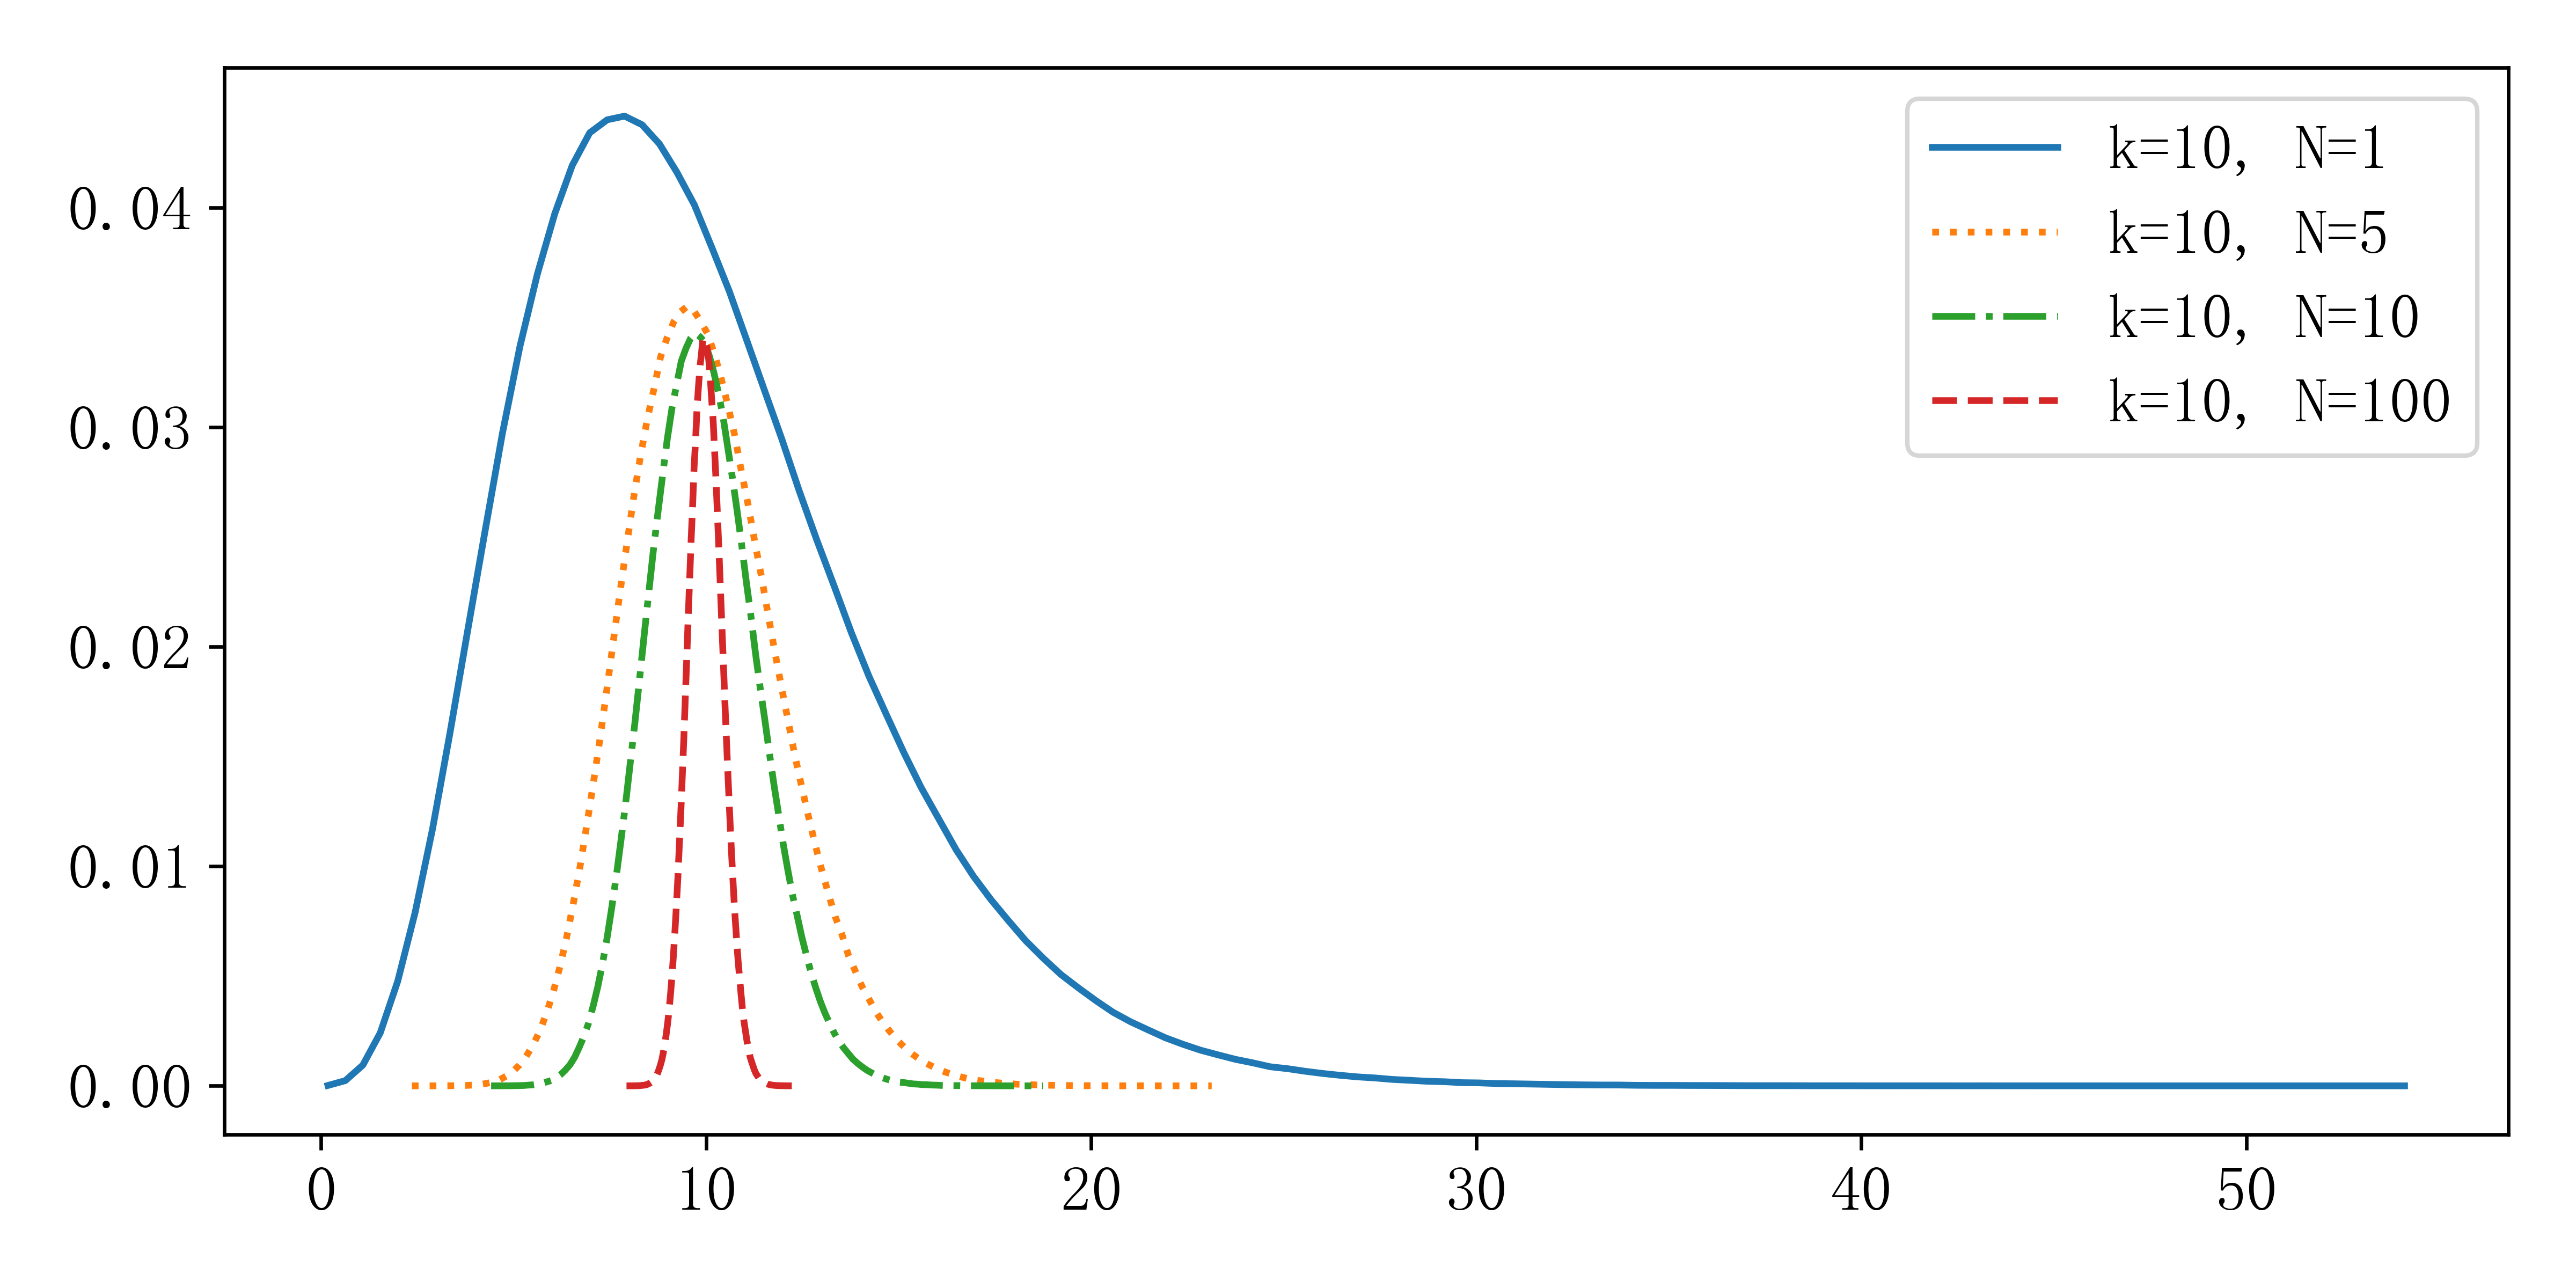
\includegraphics[scale=0.8]{C:/wty-yy/Code/Statistic/pg1.png}
    \caption{第一题}
\end{figure}
\begin{figure}[htbp]
    \centering
    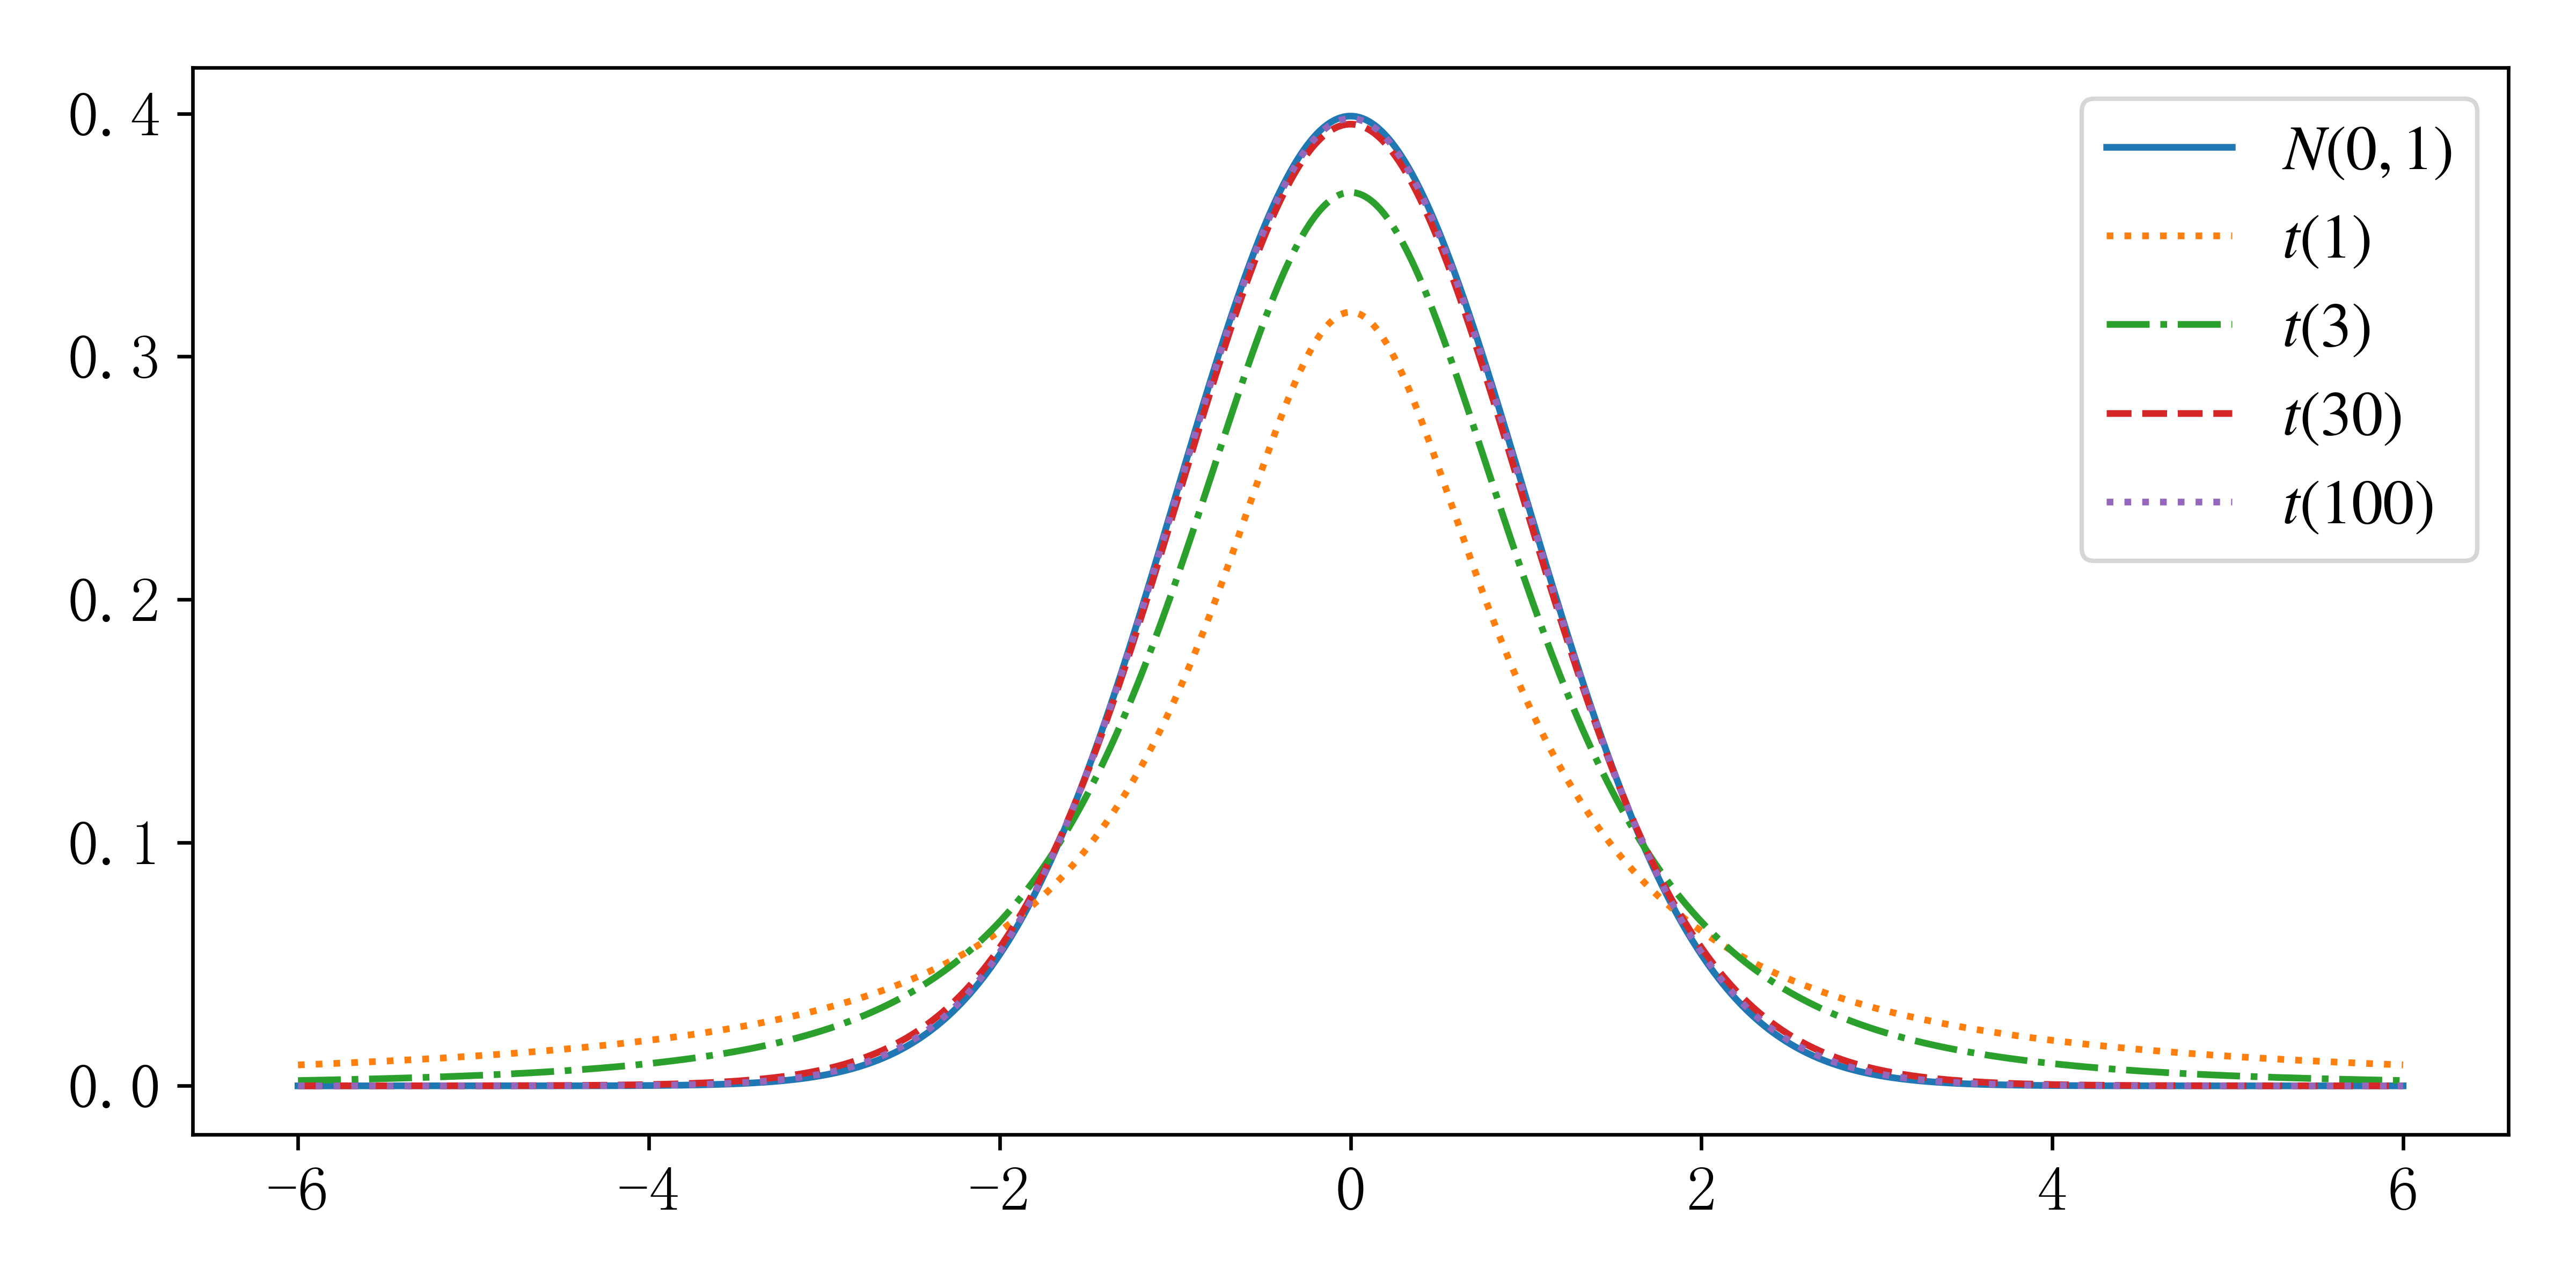
\includegraphics[scale=0.8]{C:/wty-yy/Code/Statistic/pg2.png}
    \caption{第二题}
\end{figure}

% 下面给一些功能的写法
\iffalse
% 图片模板
\centerline{
    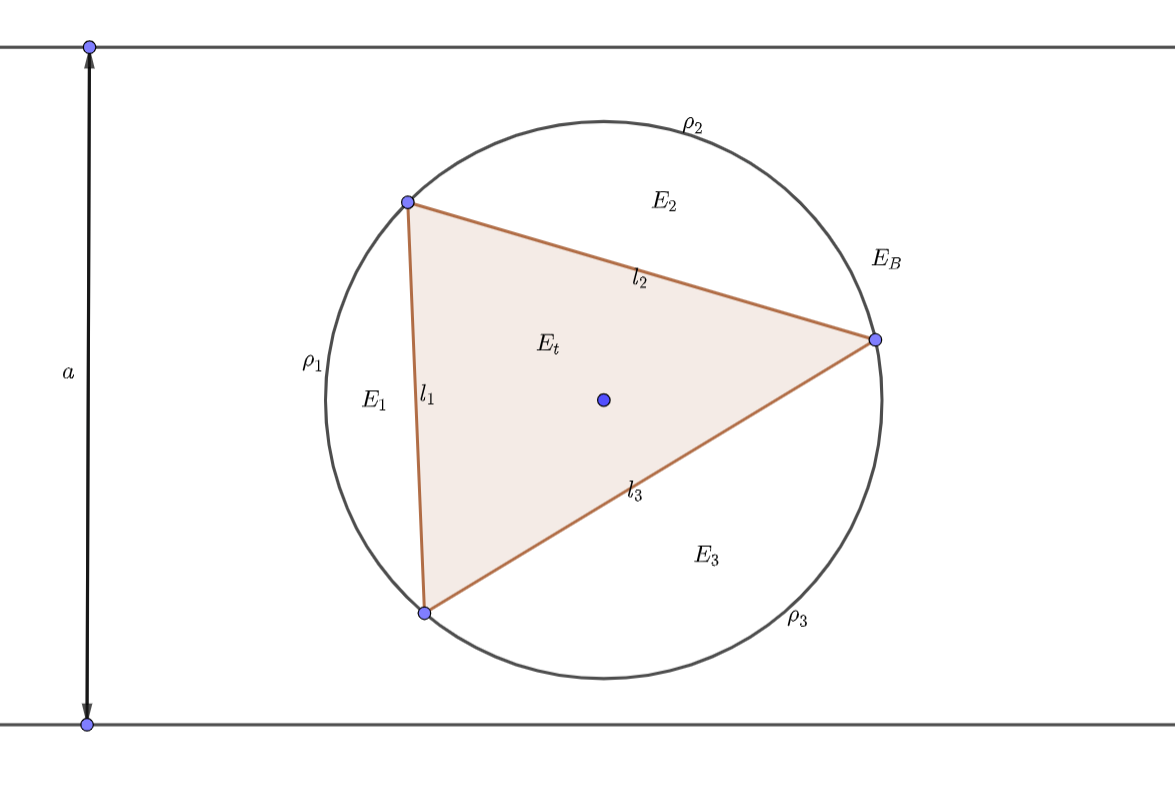
\includegraphics[width=0.8\textwidth]{figure.png}
}
% 表格模板
\renewcommand\arraystretch{0.8} % 设置表格高度为原来的0.8倍
\begin{table}[!htbp] % table标准
    \centering % 表格居中
    \begin{tabular}{p{1cm}<{\centering}p{1cm}<{\centering}p{3cm}<{\centering}p{5cm}<{\centering}} % 设置表格宽度
    %\begin{tabular}{cccc}
        \toprule
        $x_i$ & $f[x_1]$ & $f[x_i,x_{i+1}]$ & $f[x_i,x_{i+1},x_{i+2}]$ \\
        \midrule
        $x_0$ & $f(x_0)$ &                  &                          \\
        $x_0$ & $f(x_0)$ & $f'(x_0)$        &                          \\
        $x_0$ & $f(x_1)$ & $\frac{f(x_1)-f(x_0)}{x_1-x_0}$ & $\frac{f(x_1)-f(x_0)}{(x_1-x_0)^2}-\frac{f'(x_0)}{x_1-x_0}$\\
        \bottomrule
    \end{tabular}
\end{table}

\def\Log{\text{Log}} % 一个简单的宏定义
$\Log$ % 调用方法
\fi

\end{document}